\documentclass[12pt]{article}
\usepackage{verbatim}
\usepackage[dvips]{epsfig}
\usepackage[dvipsnames,usenames]{color}
\usepackage{url}
\usepackage[colorlinks=true]{hyperref}
\usepackage{enumitem} % [noitemsep,nolistsep] compact itemize/enumerate etc.
\usepackage[compact]{titlesec}
\usepackage[margin=2cm]{geometry}

% Typeface
\usepackage[condensed,math]{iwona}
\usepackage[T1]{fontenc}

% Remove spacing following headings, ie. implement \usepackage[compact]{titlesec}
%\titlespacing{\section}{0pt}{*0}{*0}
%\titlespacing{\subsection}{0pt}{*0}{*0}
%\titlespacing{\subsubsection}{0pt}{*0}{*0}

% Remove section numbering
%\setcounter{secnumdepth}{0}

% Inter-repository linking
\newcommand{\heterarchxref}[2]{\href{#1}{#2}}

 % Generate a nicely located tilde
\newcommand{\mytilde}{\raise.17ex\hbox{$\scriptstyle\mathtt{\sim}$}}
\begin{document}

\section*{HETERARCH: Technical}

{\bf Related Documentation:}
% start: userdocs-tag-replace-items related-do-nothing
% end: userdocs-tag-replace-items related-do-nothing

\section*{HCMS Version Control}

Version control of the {\bf\small{Heterarch}} content management system is currently handled by the monotone software package. Monotone is a distributed version control tool that can help automate many tedious and error-prone tasks in group software development, e.g.
\begin{itemize}[noitemsep,nolistsep]
\item Store multiple versions of files you are working on efficiently.
\item Transmit changes to files between you and your colleagues.
\item Merge changes you make with those your colleagues make.
\item Make notes about your opinion of the quality of versions of files.
\item Make decisions about using or ignoring versions, depending on the notes you receive from others. 
\end{itemize}
Please be aware that distributed version control is a feild that is currently being intensively researched and as a consequence is constantly undergoing change.

Although monotone is a slightly unorthodox version control tool, with many of its concepts similar--but subtly or significantly different--from concepts with similar names in other version control tools, it was selected because of its simple user interface.

Monotone provides a simple, single-file transactional version store, with fully disconnected operation and an efficient peer-to-peer synchronization protocol. it understands history-sensitive merging, lightweight branches, integrated code review and 3rd party testing. It uses cryptographic version naming and client-side RSA certificates. It has good internationalization support, has no external dependencies and runs on Linux, Solaris, OSX, Windows, and other Unixes.

\subsection*{Obtaining Monotone}
Monotone can be obtained by downloading the package appropriate for your computing platform from the links on the \href{http://monotone.ca/}{\bf monotone} home page.

%\subsection*{Installing Monotone on OS X}
%On the monotone home page select the Mac OS X packaged link and download the DMG file.

\subsection*{Manual Monotone Initialization}

Once the appropriate monotone package has been downloaded and installed on your computer, monotone must be initialized by performing the following steps (commands in the monospaced {\tt typewriter} font should be entered from a Terminal command line prompt):

\begin{enumerate}

\item {\bf Generate a monotone key:} 
\begin{verbatim}
    mtn genkey <identifier>
\end{verbatim}
where the {\tt $<$identifier$>$} is unique to you (typically an email account, e.g. yourname@provider). The identifier is located in a {\it .monotone} directory in your home folder located in the {\it /Users} folder.

\item {\bf Initialize the data base}
\begin{verbatim}
    mtn --db=userdocs.mtn db init
\end{verbatim}
This creates the monotone repository file {\it userdocs.mtn} which is referenced with
\begin{verbatim}
    --db=userdocs.mtn
\end{verbatim}

\item {\bf Create a workspace}
\begin{verbatim}
    mtn --db=userdocs.mtn --branch="0" setup userdocs
\end{verbatim}
This creates a workspace directory on your local machine where you put the source files for any documentation that you create. Importantly, there is a specific required structure and content for documents in the {\bf\small{Heterarch}} content management system that is described in \href{../document-create/document-create.tex}{\bf Create\,a\,Document}. The path to the workspace directory should be
\begin{verbatim}
    ~/neurospaces_project/userdocs/source/snapshots/0
\end{verbatim}
By default, the workspace directory {\tt 0} contains a folder named {\tt \_MTN}. This is part of the monotone version control system and contains information concerning monotone's version control management.

The command
\begin{verbatim}
    mtn --db=userdocs.mtn pubkey <identifier> > me.pubkey
\end{verbatim}
will place a copy of your public key in the file indicated in {\tt --db=userdocs.mtn}.
\end{enumerate}
An automatic login can be set up with monotone by making an executable file containing the following code:
\begin{verbatim}
    ~/.monotone/monotonerc:
        function get_password(keypair_id)
        return <password here>
        end

\end{verbatim}
Further information and help about using monotone, for example resolving conflicts between documents, can be found at:

\href{http://monotone.ca/monotone.html}{\bf http://monotone.ca/monotone.html}.

\section*{Heterarch and the Monotone Version Control System}

Installation and maintenance of the {\bf\small{Heterarch}} Content Management System is fully automated with document versioning under the control of \href{http://monotone.ca/}{\bf monotone}. 

\subsection*{Overview}

In its simplest form, the {\bf\small{Heterarch}} content management version control system can be seen as having three levels (see figure below):
\begin{enumerate}

\item {\bf The local documentation workspace:} Exists at a specified location within the {\bf\small{Heterarch}} developers installation on your local machine. The contents of this workspace are private to the local filesystem.

\item {\bf The private document repository:} Provides the first step in document publication. Documentation version control is initiated by checking documents in your local workspace into the document repository on your local machine.

\item {\bf The public document repository:} Pushing documents from your local repository to the publicly accessible repository makes all documentation in your local repository available (i) for publication on a {\bf\small{Heterarch}} website and (ii) to become part of the {\bf\small{Heterarch}} content management system that can optionally be downloaded as part of a {\bf\small{Heterarch}} installation. It also allows other members of your development team to work simultaneously on documentation.

\end{enumerate}

\begin{figure}[h]
  \centering
 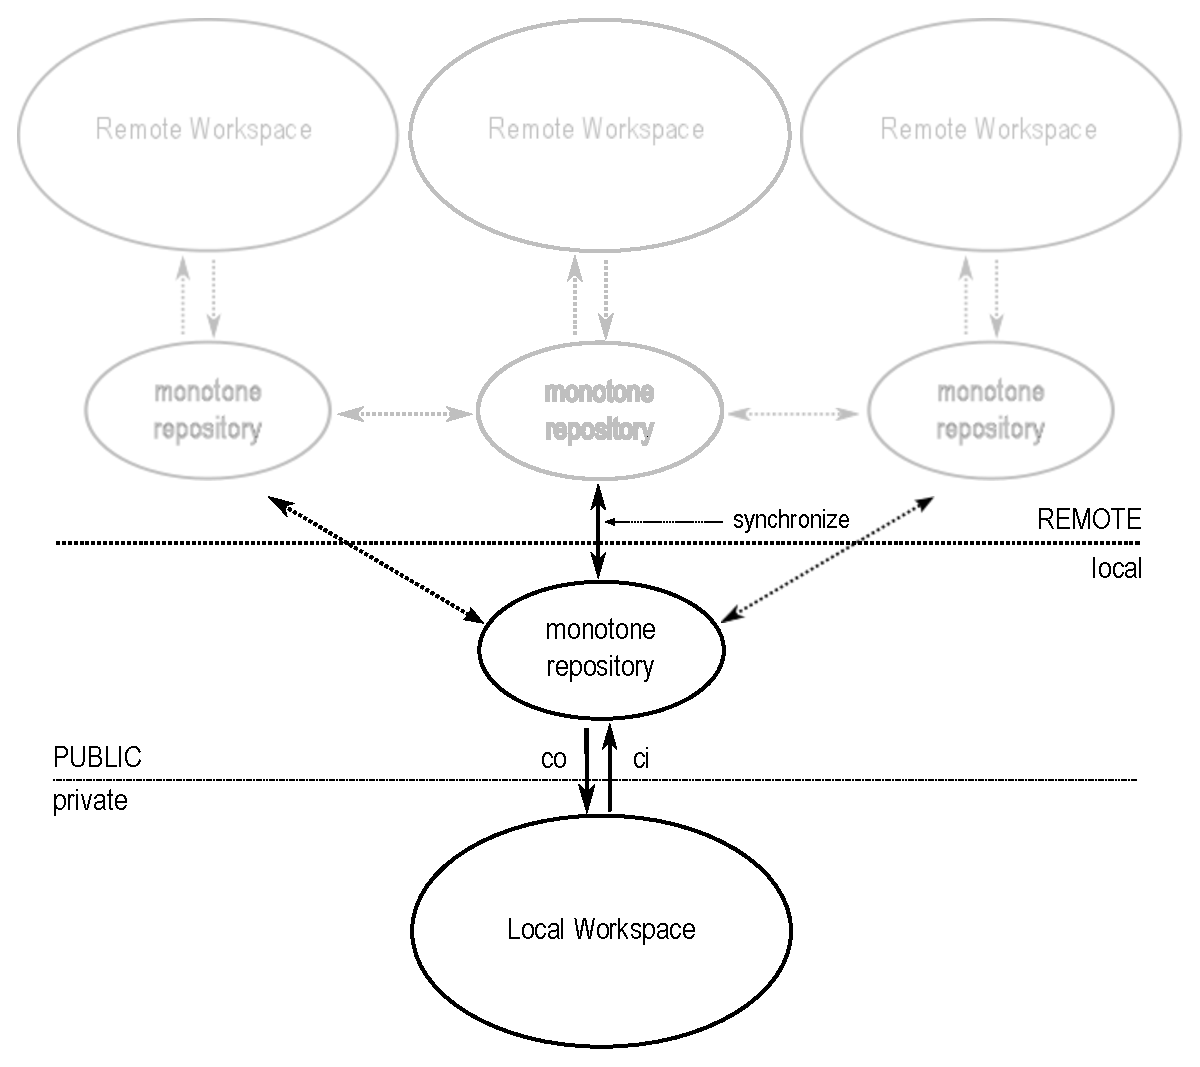
\includegraphics[scale=0.6]{figures/heterarch-monotone.eps}
%  \caption{}
  \label{fig:monotone}
\end{figure}

The components of the monotone version control system are illustrated in the above figure. It shows the relationship between a local workspace, its associated monotone repository, and how after an initial ``check in'' ({\it ci}), a document can be ``pushed'' to the monotone server database that forms a monotone repository. Note that documents are private to your local account until they are pushed to the monotone server. At this point they become available to other registered users of the monotone system.

Once a document is located on the monotone server repository, it is available to be published as part of the {\bf\small{Heterarch}} content management system. This means that it will be automatically incorporated and downloaded as part of the {\it userdocs} module when {\bf\small{Heterarch}} is installed or updated.

\subsection*{Monotone Workflow Examples}

The following sections give some example workflows for monotone use. More detailed tutorials and documentation are available from the \href{http://www.monotone.ca/docs/index.html}{\bf monotone} website.

\subsection*{Updating the Local Workspace}

Updating your local workspace begins with determining which files are registered with monotone. This is done by querying your local monotone repository. This generates a list of any new files that may have been added to your local work space since the last update
\begin{verbatim}
    mtn ls unknown
\end{verbatim}
This command generates a list of all files in your local workspace that are not known to monotone. To have any files that this command lists added to your local repository, enter:
\begin{verbatim}
    mtn add --unknown
\end{verbatim}
Reissuing the ``{\tt mtn ls unknown}'' command should now result in no output.

Alternatively, once files have been registered in your local workspace, the following command reports which have been changed since the last code check in (see following):
\begin{verbatim}
   mtn ls changed
\end{verbatim}

Importantly, the default file type for the {\bf\small{Heterarch}} Content Management System is the \LaTeX2e\,\,{\bf .tex} file. To register a different file type with monotone and add it to your local workspace, for example a PDF file (see \href{../common-suffixes/common-suffixes.tex}{\bf Common\,Suffixes} for a more complete list of recognized file types), use the following command:
\begin{verbatim}
   mtn add --no-respect-ignore <directory-name>/<file-name>.pdf
\end{verbatim}

The files that have been registered with monotone can now be added to your local repository with the following command:
\begin{verbatim}
    mtn ci
\end{verbatim}
where {\tt ci} stands for ``check in''. Monotone responds by opening the log file indicated in {\tt .\,--db=heterarch.mtn} where the nature of the changes or revision to the document(s) that are being checked in can be recorded.

\subsection*{Synchronizing the Local Workspace with the Monotone Repository}

The following procedure is suggested for syncing with repository at the end of each day and/or documentation writing session.

\begin{verbatim}
    mtn ls unknown
        . . .
    mtn add --unknown
\end{verbatim}
These commands add any new files discovered in your local workspace to your local monotone repository. That this has occurred correctly can be checked with
\begin{verbatim}
    mtn ls known .
\end{verbatim}
This command should generate the same list of file names as that returned by the ``{\tt mtn ls unknown}'' command. Note the period ``{\tt .}'' which is part of the command syntax.

You can then check for files in you local workspace that have been deleted or moved
\begin{verbatim}
    mtn ls missing
\end{verbatim}
You can then drop any files missing from your local workspace repository by entering:
\begin{verbatim}
    mtn drop --missing
\end{verbatim}
and then check in the changes to the monotone repository on the server with
\begin{verbatim}
    mtn ci
\end{verbatim}
You can automate the synchronization of your local data base (i.e. a push and a pull) with the monotone repository on the server by placing an executable file (named for example,\,{\it <repository-name>-sync}) in a bin directory in your local work space, e.g. {\it neurospaces\_project/<repository-name>/source/snapshots/0/bin}. 
The executable contains the command sequence:
\begin{verbatim}
    neurospaces_sync --enable <repository-name> --regex <repository-name> --verbose
\end{verbatim}
and issuing the command
\begin{verbatim}
   <repository-name>-sync
\end{verbatim}
simultaneously updates the monotone repository on the server and transfers any updates to documentation on the server to your local monotone repository. Once this has been done, the files that have been pushed to the monotone server are available for other registered users to pull down to their own local monotone repository and to check them out ({\it co}) to their local workspace.

\subsection*{File Recovery}

The latest version of a file can be recovered with the following command
\begin{verbatim}
   mtn revert <file name> .
\end{verbatim}

\end{document}